\documentclass[11pt]{article}

\usepackage{common}
\usepackage{amsmath}
\DeclareMathOperator*{\E}{\mathbb{E}}

\title{HW2: Language Modeling}
\author{Emily Tseng \\ et397@cornell.edu}
\begin{document}

\maketitle{}
\section{Introduction}

In a sense, a language is just a set of community-driven rules for what words should appear in what order. Language modeling is a generative problem that attempts to formalize this ordering by computing a probability distribution over a given sequence. As an example, consider the incomplete sentence ``\textit{Tickets were sold out for the 2 p.m. \_\_\_\_\_}'' A language model properly trained over the English language would compute a greater probability for the sentence ending in ``\textit{movie}'' than, say, the sentence ending in ``\textit{banana}''. 

The key is to generate a distribution as close as possible to the true distribution of your source language; or, in empirical terms, to maximize the probability (or minimize the perplexity) of the sentences in your test set. In this homework, we use data from the Penn Treebank \citep{marcus-etal-1993-building} to implement, train and assess several varieties of language models:

\begin{enumerate}
  \item A count-based trigram model with linear interpolation
  \item A neural network language model \citep{bengio2003neural}
  \item A Long Short-Term Memory (LSTM) language model \citep{zaremba2014recurrent}
\end{enumerate}

For each of the above models, we report perplexity on the validation and testing sets. We additionally consider the following two extensions:

\begin{enumerate}
  \item Consider 3-4 train and test contexts and do an information-theoretic analysis of the output of the model. What is the entropy of the distribution? What is the KL between different models, and what does this tell us about the predictions and the contexts?
  \item Formulate an EM algorithm for estimating $\alpha$ for the count-based model. That is, imagine there is a latent Z categorical variable over three choices, where $p(Z)$ is a prior prob of using a unigram, bigram, or trigram model. This formulation is identical to the one above, but allows us to learn the $\alpha$ values using EM. The approach has two steps: Start with random alpha, 1) Learn a model with that alpha, 2) *On validation* compute $p(z_t | x_t, x_{t-1}, x_{t-2})$ for each position to use as new alphas. 
\end{enumerate}

\section{Problem Description}

Consider a sentence as a sequence of tokens $x_{1:T}$ for a sentence of length $T$ where all tokens are drawn from the same unigram distribution $V$. In a given language, the probability of the sentence can be described as:
\begin{align*}
  p(x_{1:T}) = \prod_{i=1}^{T} p(x_{T} | x_1 ... x_{T-1})
\end{align*}

The goal of a language model is to estimate a distribution that maximizes the probabilities of the sentences in a provided test set. From information theory, we have the following ways to quantify a distribution: \textit{entropy} ($H$), a measure of deviance from the uniform distribution, and \textit{perplexity} ($PP$), the exponentiated entropy of a distribution and the measure commonly used in NLP. Formally defined, for a distribution $p$ with observations $x \in X$:
\begin{align*}
  H(p) &= - \sum_{i} p(x=i) \log[p(x=i)] \\
       &= - \E_{x\in p} \log[p(x)] \\
  PP(p) &= \exp{H(p)} 
\end{align*}

The goal of this assignment will be to train language models that mimic the perplexities reported in the source papers as closely as possible.

% In general, homeworks will be specified using informal
% language. As part of the assignment, we expect you to write-out a
% definition of the problem and your model in formal language. For this
% class, we will use the following notation:

% \begin{itemize}
% \item $\boldb, \boldm$;  bold letters for vectors.
% \item $\boldB, \boldM$;  bold capital letters for matrices.
% \item $\mcB, \mcM$;  script-case for sets.
% \item $b_i, x_i$; lower case for scalars or indexing into vectors.
% \end{itemize}


% For instance in natural language processing, it is common to use
% discrete sets like $\mcV$ for the vocabulary of the language, or $\mcT$ for a
% tag set of the language.  We might also want one-hot vectors
% representing words. These will be of the type
% $\boldv \in \{0,1\}^{|\mcV|}$. In a note, it is crucial to define the
% types of all variables that are introduced. The problem description is the
% right place to do this.

% NLP is also
% full of sequences. For instance sentences, $w_1, \ldots, w_N$, where
% here $N$ is a constant length and $w_i \in \mcV$ for all
% $i \in \{1, \ldots N\}$. If we pretend sentences are all the same
% length, we can have scoring function over sentences,
% $s : \mcV^N \mapsto \reals$.  One might be defined as:

% \[ s(w_1, \ldots, w_N) = \sum_{i = 1}^N p(w_i | w_{i-2}, w_{i-1}), \]

% \noindent where $p$ is the bigram probability, which we will cover later in the class.

\section{Model and Algorithms}

\subsection{Count-based Trigram Model with Linear Interpolation}

$$p(y_t | y_{1:t-1}) =  \alpha_1 p(y_t | y_{t-2}, y_{t-1}) + \alpha_2 p(y_t | y_{t-1}) + (1 - \alpha_1 - \alpha_2) p(y_t) $$

\subsection{EM Algorithm for $a$ Estimation}

\subsection{Neural Network Language Model}

\subsection{LSTM Language Model}


% \begin{itemize}
% \item diagrams of your model,

%   \begin{center}
%     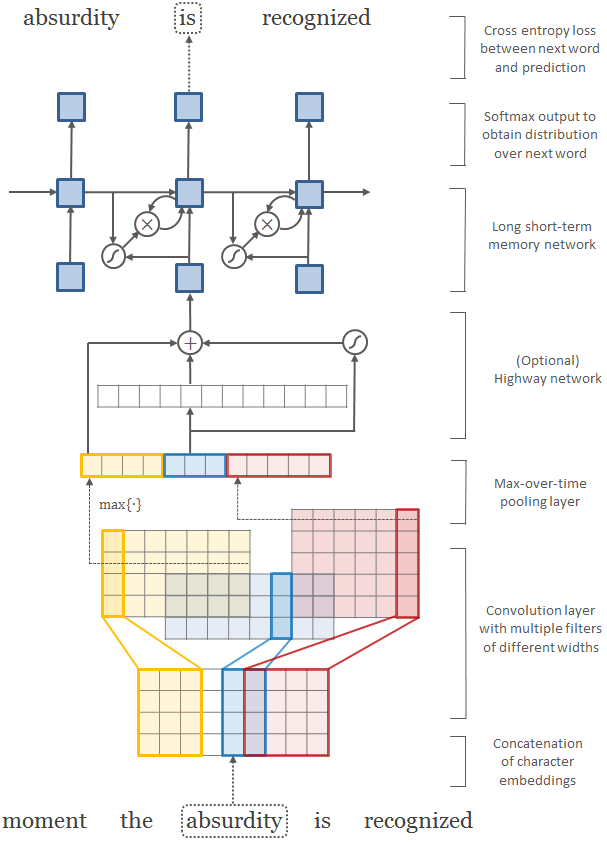
\includegraphics[width=0.4\textwidth]{network}
%   \end{center}
% \item feature tables,

%   \begin{center}
%     \begin{tabular}{@{}lll@{}}
%       \toprule
%       &\multicolumn{2}{c}{Mention Features  } \\
%       & Feature & Value Set\\
%       \midrule
%       & Mention Head & $\mcV$ \\
%       & Mention First Word & $\mcV$ \\
%       & Mention Last Word & $\mcV$ \\
%       & Word Preceding Mention & $\mcV$ \\
%       & Word Following Mention & $\mcV$\\
%       & \# Words in Mention & $\{1, 2, \ldots \}$ \\
%       & Mention Type & $\mathcal{T}$ \\
%       \bottomrule
%     \end{tabular}
%   \end{center}

% \item pseudo-code,

%   \begin{algorithmic}[1]
%     \Procedure{Linearize}{$x_1\ldots x_N$, $K$, $g$}
%     \State{$B_0 \gets \langle (\langle \rangle, \{1, \ldots, N\}, 0, \boldh_0, \mathbf{0})  \rangle$}
%     \For{$m = 0, \ldots, M-1$ }
%     \For{$k = 1, \ldots, |B_m|$}
%     \For{$i \in \mcR$}
%     \State{$(y, \mcR, s, \boldh) \gets \mathrm{copy}(B_m^{(k)})$}
%     \For{word $w$ in phrase $x_i$}
%     \State{$y \gets y $ append $w$ }
%     \State{$s \gets s + \log q(w, \boldh) $ }
%     \State{$\boldh \gets \delta(w, \boldh)$}
%     \EndFor{}
%     \State{$B_{m+|w_i|} \gets B_{m+|w_i|} + (y, \mcR - i, s,   \boldh)$}
%     \State{keep top-$K$ of $B_{m+|w_i|}$ by $f(x, y) + g(\mcR)$}
%     \EndFor{}
%     \EndFor{}
%     \EndFor{}
%     \State{\Return{$B_{M}^{(k)}$}}
%     \EndProcedure{}
%   \end{algorithmic}

% \end{itemize}


\section{Experiments}

% Finally we end with the experimental section. Each assignment will make clear the main experiments and baselines that you should run. For these experiments you should present a main results table. Here we give a sample Table~\ref{tab:results}. In addition to these results you should describe in words what the table shows and the relative performance of the models.

% Besides the main results we will also ask you to present other results
% comparing particular aspects of the models. For instance, for word
% embedding experiments, we may ask you to show a chart of the projected
% word vectors. This experiment will lead to something like
% Figure~\ref{fig:clusters}. This should also be described within the
% body of the text itself.


% \begin{table}[h]
% \centering
% \begin{tabular}{llr}
%  \toprule
%  Model &  & Acc. \\
%  \midrule
%  \textsc{Baseline 1} & & 0.45\\
%  \textsc{Baseline 2} & & 2.59 \\
%  \textsc{Model 1} & & 10.59  \\
%  \textsc{Model 2} & &13.42 \\
%  \textsc{Model 3} & & 7.49\\
%  \bottomrule
% \end{tabular}
% \caption{\label{tab:results} Table with the main results.}
% \end{table}


% \begin{figure}
%   \centering
%   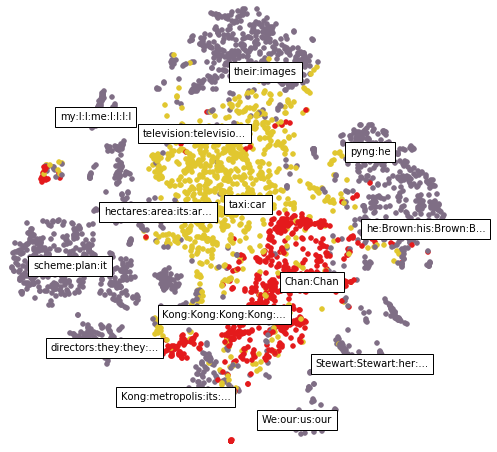
\includegraphics[width=6cm]{cluster_viz}
%   \caption{\label{fig:clusters} Sample qualitative chart.}
% \end{figure}


\section{Conclusion}

End the write-up with a very short recap of the main experiments and the main results. Describe any challenges you may have faced, and what could have been improved in the model.

\bibliographystyle{apalike}
\bibliography{hw2-writeup}

\end{document}
